This section describes the implementation of SESH into SAMMY as required for fitting resonance parameters to self-shielded URR measurements.

\section{URR Representation in SAMMY}

The average cross section in the URR is typically defined according to Hauser-Feshbach theory, which provides a framework for describing nuclear reactions proceeding through a compound nucleus when many channels are open and individual resonance effects are smeared out. The energy-averaged total cross section for an incoming channel $c$ can be expressed as:

\begin{equation}
    \label{eq:hauser-feshbach-cross-section}
    \langle \sigma_c \rangle =
    2 \pi \lambdabar_c^2 g_c \left\{
    1 - \frac{
            \cos{ ( 2 \phi_c)} \left[
                1 - \pi^2P_c^2 s_c^2 -  \left( P_c R_c^\infty \right)^2
            \right]
            + \sin{(2 \phi_c)} 2 P_c R_c^\infty
        }{
            \left( 1 + \pi P_c s_c \right)^2 + \left( P_c R_c^\infty \right)^2
    }
    \right\} \quad \text{}
\end{equation}
In this formulation, $\lambdabar$ is the reduced de Broglie wavelength for the neutron, $g_c$ is the statistical spin factor defined as $g_c = \frac{2J + 1}{2(2I + 1)}$ where $I$ is the spin of the target nucleus , and $\phi_c$ is the hard-sphere scattering phase shift for a particular channel. The form of $\phi_c$ depends on the orbital momentum $\ell$ and is a function of $\rho = \frac{a_c}{\lambdabar}$, where $a_c$ is the scattering radius of the target nucleus.

The parameters of significance to transmission self-shielding in the URR, which distinguish this average cross section from a simple energy average of RRR cross sections, are the distant level parameter $R^\infty_c$ and the strength function $\Tilde{S}_c$. Here, $P_c$ is the neutron penetrability, and $s_c$ is the pole strength, defined as $s_c = \Tilde{S}_c\lambdabar a_c \sqrt{E}/2$. The strength function $\Tilde{S}_c$ characterizes the average reduced width of resonances for a given orbital $\ell$.


\section{Converting from SAMMY Parameters to SESH Parameters}
    \subsection{Calculating Available Channels}

    As mentioned in the previous section, the relevant URR parameters are all given only as their $\ell$ basis. As a requirement for simulating resonances for calculating resonance self-shielding, these parameters need to be calculated according to $(J,\ell,\pi)$ rather than just $\ell$ dependencies.

    For an isotope with a ground-state spin $I$ interacting with a neutron (which has an intrinsic spin of $s_n = 1/2$), there are two possible channel spins: $s_{-} = I - 1/2$ and $s_{+} = I + 1/2$. This leads to two separate cases for the total angular momentum $J$: one for $s_{-}$ and one for $s_{+}$:
    \begin{align}
        J_{-} &= \left\{ \left|s_{-} - \ell\right|, \left|s_{-} - \ell\right| + 1, \cdots, s_{-} + \ell \right\}\\
        J_{+} &= \left\{ \left|s_{+} - \ell\right|, \left|s_{+} - \ell\right| + 1, \cdots, s_{+} + \ell \right\}
    \end{align}
    One common assumption is that spin-group parameters are assumed to be independent of parity, i.e., $(J, \ell, -1) = (J, \ell +1)$. As a consequence, only $J$ and $\ell$ need to be considered when calculating resonances. Instead, the important factor to consider is the degrees of freedom, or the multiplicity, $\mu$. If the same $J,\ell$ combination can be calculated from $s_{+}$ and $s_{-}$ channel spins, then $\mu_i = 2$. Otherwise, $\mu_i=1$.

    \begin{equation}
        \begin{array}{rrrrrrrr}
J_{-}: & \{ & \left|s_{-} - \ell\right|, & \left|s_{-} - \ell\right| + 1, & \dots, & s_{-} + \ell ~ & & \} \\
J_{+}: & \{ & & \left|s_{+} - \ell\right|, & \dots, & s_{+} + \ell-1, & s_{+} + \ell & \} \\[1em] \hline \\[-0.5em]
\mu_J: & \{& 1, & 2, & \dots, & 2, & 1 & \} \\
\end{array}
    \end{equation}

    \subsection{Converting from $R^\infty$ to $R'$}

    \subsection{Converting Inelastic Strength to Inelastic Widths from Channels}

\section{Improving Level Density Energy Dependency}

\section{Doppler Broadening Bug}
    The primary cause of the disagreement was determined to be the result of an error in the Doppler broadening subroutine that was originally present in SESH. In order to perform the Doppler broadening, the complex error function, also known as the Faddeeva function, is utilized. The issue was in the original algorithm, in cases where $\beta$ was less than 0.01. Recall that
    \begin{equation}
        w(\alpha,\beta) = \frac{i}{\pi} \int_{-\infty}^{\infty} \frac{e^{-t^2}}{\alpha + i\beta - t}dt
    \end{equation}
    and
    \begin{equation}
        \beta = \frac{\theta}{2} = \frac{\Gamma_{tot}}{4\sqrt{\frac{ \kappa T E}{A}}}
        \label{eq:doppler-beta}
    \end{equation}

    In instances where $\beta \leq 0.01$, the algorithm would incorrectly return the 0 Kelvin value for the $\psi$ parameter, shown in \autoref{fig:beta-error}.
    \begin{figure}
        \centering
        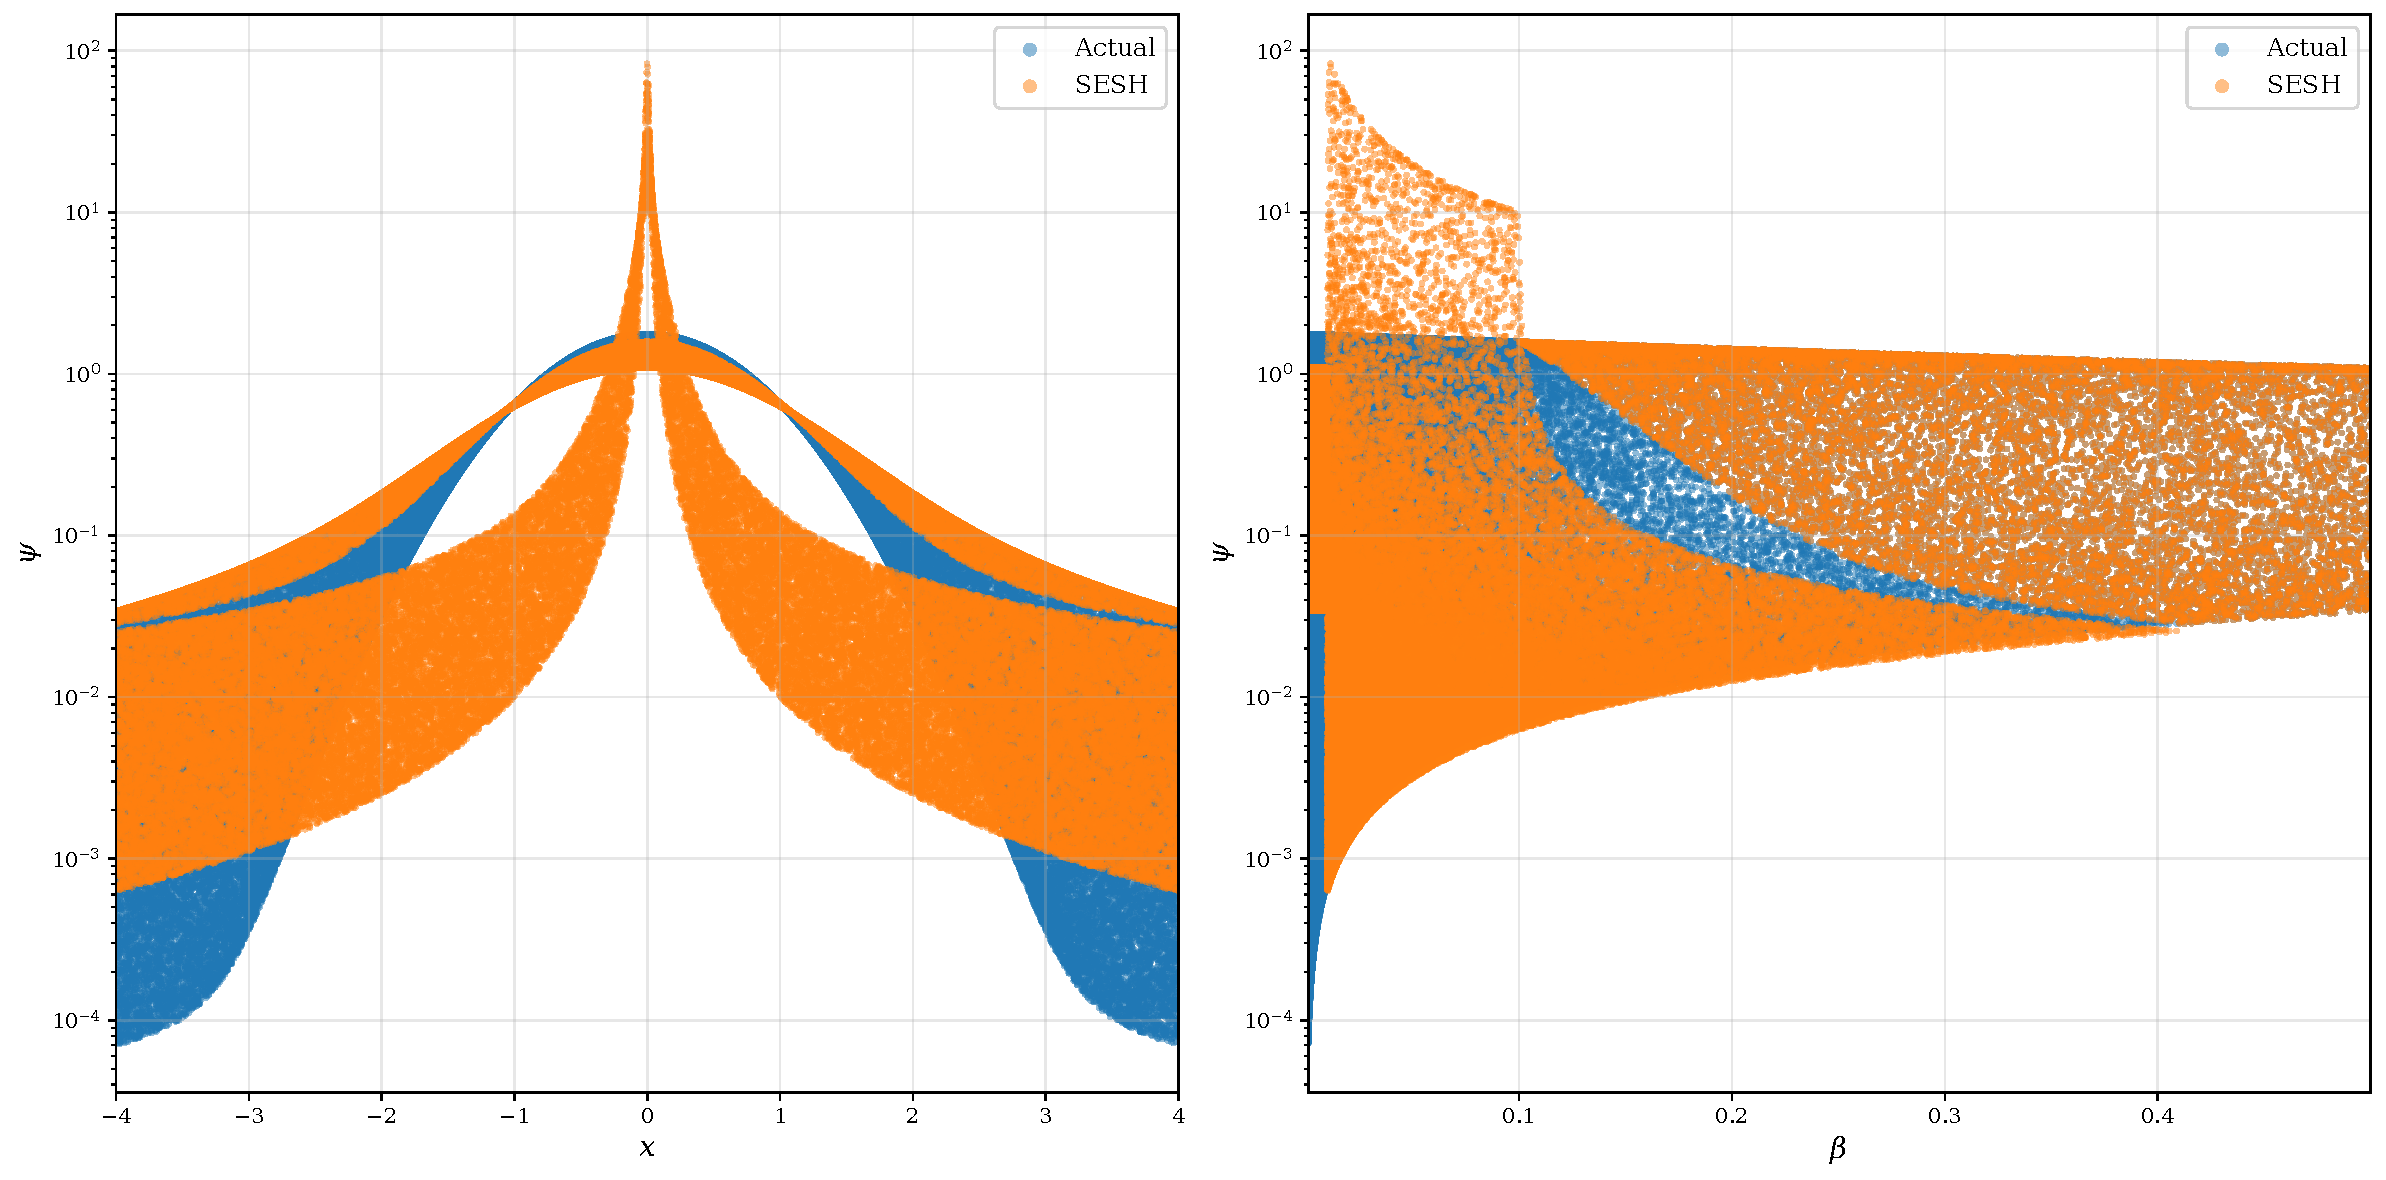
\includegraphics[width=0.95\linewidth]{Implementation/Figures/beta-error.png}
        \caption{Comparing results of SESH's Faddeeva function output with what the Faddeeva function actually calculates given the same inputs.}
        \label{fig:beta-error}
    \end{figure}
    
    One significant effect of this bug is due to the inverse relationship between $\beta$ and energy, shown in \autoref{eq:doppler-beta}. As the energy of the incident neutron increases, the probability of $\beta$ being sampled as less than 0.01 increases. Consequently, as energy increases, the probability of the 0 Kelvin cross section being returned also increased.

\section{Energy Deposition Improvement}
    Originally in SESH, there was a very simple approximation for sampling what energy an interaction occurred at. It was assumed that every neutron lost the average scattering energy per collision, independent of scattering angle, i.e.,
    \begin{equation}
        E' = E \left[ 1 - \frac{2A}{\left( 1 + A \right)^2} \right]
    \end{equation}
    for all post-collision neutrons. This enabled all of the energy dependent parameters that did not get sampled using the Monte Carlo method to be pre-calculated efficiently. However, it was assumed this would be an insufficient approximation for thick samples in which many collisions were expected.
    
    This was substituted with an angle-dependent energy sampling procedure. The scattering angle of each post collision neutron would be sampled assuming an isotropic scattering distribution, and the post collision energy would be calculated as a function of the scattering angle,
    \begin{equation}
        E' = E \frac{A^2 + 2 A \mu_c + 1}{\left( A + 1 \right)^2}
    \end{equation}
    in which
    \begin{equation}
        \mu_c = \cos\phi_c
    \end{equation}
    where $\phi_c$ is the exit angle of the post-collision neutron in the center-of-mass system.
    \begin{figure}
        \centering
        \includegraphics[width=0.95\linewidth]{Implementation/Figures/multiple_scattering.png}
        \caption{Distribution of neutrons after each collision using the old SESH post-collision energy sampling method and the new angle-dependent sampling in a 12mm \textsuperscript{181}Ta sample at 3keV initial incident energy.}
        \label{fig:multiple-scattering}
    \end{figure}